\chapter{Omnidirectional interferometry}\label{ch:omnidirectional}
Parts of this chapter have been submitted as Kagias M, Abis M, Wang Z,
Jefimovs K, Stampanoni M,
\emph{Generalized omnidirectional scattering sensitivity}. My contributions
to this work concern the installation and adaptation of an omnidirectional scattering
system~\parencite{PhysRevLett.116.093902} on a laboratory source.

\section{Introduction}
The Talbot-Lau interferometer described in chapter~\ref{ch:review} is one
method of exploiting the self-imaging phenomenon for a periodical wave in
order to transform phase differences into intensity modulations.
An alternative approach has been established on synchrotron
sources~\parencite{PhysRevLett.116.093902} in order to overcome two limitations
of conventional grating interferometry: first, the limitation of the sensitivity of
the phase and dark-field signals to the direction orthogonal to the grating
lines (equation~\ref{eq:talbot1}); second, the phase stepping procedure, where
the analyzer grating is scanned across the interference fringes in order to
decode the three characteristic signals
(section~\ref{sec:gi-image-analysis}), which requires multiple exposures and
a precise displacement of the absorption grating \G2 of the order of
hundreds of nanometers.

The setup proposed in~\parencite{PhysRevLett.116.093902} relies on the modulation
of a wave front that is periodical in two ways: a unit cell made of
concentric circles introducing a phase shift of $\pi/2$ in the X-rays,
replicated across the field of view
(figure~\ref{fig:omnidirectional-synchrotron}).

\begin{figure}[htb]
    \centering
    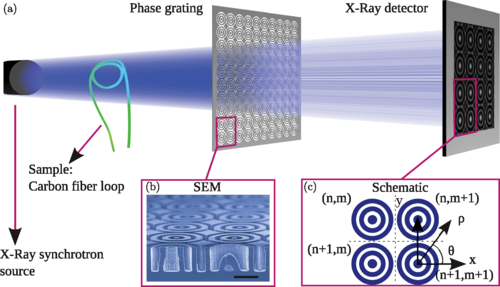
\includegraphics[width=\textwidth]{gfx/omnidirectional/synchrotron-design.png}
    \caption[Synchrotron experimental setup for omnidirectional grating
    interferometry.]{Experimental setup for a synchrotron omnidirectional grating
    interferometer. The unit cells with concentric circles are shown in the
    \ac{SEM} image and in the recorded interference fringe. Reprinted figure
with permission from Kagias M, Wang Z, Villanueva-Perez P, Jefimovs K,
Stampanoni M, \emph{2D-Omnidirectional Hard-X-Ray Scattering Sensitivity in
a Single Shot}, Phys. Rev. Lett. 116, 9, 093902, 2016. Copyright 2016 by the
American Physical Society.}
    \label{fig:omnidirectional-synchrotron}
\end{figure}

The key feature is the self-imaging of the circular structures 
at the Talbot distances, again according to
equation~\ref{eq:talbot.distance}:
\begin{equation*}
    \Delta_n = n \frac{p_1^2}{2 \lambda} \qquad n \in
    \mathbb{N}.
\end{equation*}
Additional imperfections are introduced by the finite number of periods in
each unit cell, but these are smoothened out as a result of the finite
source size as reported in~\cite{PhysRevLett.116.093902}. This is even
more so in the case of a laboratory source with a compact setup.
This pattern is replicated with a period $P$ of the unit cells themselves,
for which
\begin{equation}
    P = Np_1.
    \label{eq:unit.cell.periop}
\end{equation}
These fringes have to be large enough to be directly resolved at the
detector, as the data from neighnouring detector pixels belonging to the same
unit cell are analyzed together, resulting in a macroscopic pixel in the final image. Analogously to
the phase stepping approach for Talbot-Lau interferometry, each unit cell
records a circular interference fringe that is approximated with a sinusoid
\begin{equation}
    I(x, y) = a_0 + a_1(\theta)\cos\left(\frac{2\pi}{p_1} \sqrt{x^2 +
    y^2}\right),
    \label{eq:omnidirectional.periodical.signal}
\end{equation}
where $x$ and $y$ are the positions of the pixels with respect to the center
of the unit cell pattern, as identified by the pixel with maximum intensity,
and $\theta = \arctan(y/x)$.

Again similarly to equation~\ref{eq:flat} a comparison between a
\emph{flat} and a \emph{sample} curve with the same shape is required. The
sample will introduce a reduction in the average value $a_0$, related to the
transmission signal; a displacement of the location of the maximum $(x, y)$,
related to the refraction of the X-ray beam; and a reduction in the
visibility of the pattern $a_1$. 

The dark field signal, or visibility reduction signal, can be
determined as a function of the angle $\phi$ around the circle by
calculating the Fourier transform of the line passing through the center of
the unit circle at the angle $\phi$ and taking the ratio of the $N$-th to
the zeroth component
\begin{equation}
    B = \frac{a_{1,s}(\theta = \phi)}{a_{1,f}(\theta =
\phi)}\frac{a_{0,f}}{a_{0,s}}
    \label{eq:dark-field-omnidirectional}
\end{equation}

\section{An omnidirectional setup for laboratory sources}
These are the features of omnidirectional dark-field imaging so far reported
in~\parencite{PhysRevLett.116.093902}, our goal was to export the same
technique from a synchrotron to a conventional X-ray source.
As described in~\parencite{kagias2018omnidir}, the main problem is the
resolution of
the very fine self-image of the grating with a period in the order of 
micrometers. The detector used for this experiment in the same as in
chapter~\ref{ch:lung-dark-field}, the cadmium telluride prototype Santis
CdTe by Dectris Ltd. While this provides excellent efficiency at high
energy, its resolution of \SI{75}{\micro\meter} cannot be compared with the
submicron resolution available for the synchrotron experiment employing a tenfold optical magnification.

This issue can be overcome by designing each unit cell as a beam splitter
grating (figure~\ref{fig:beam-splitter}). The resulting intensity profile in the far
field has one central maximum, a minimum and a secondary maximum along the
radial direction away from the center. This cell
is then repeated across the field of view and the Talbot effect is then used
to form a self-image of this larger pattern with period $P$.

\begin{figure}[htb]
    \centering
    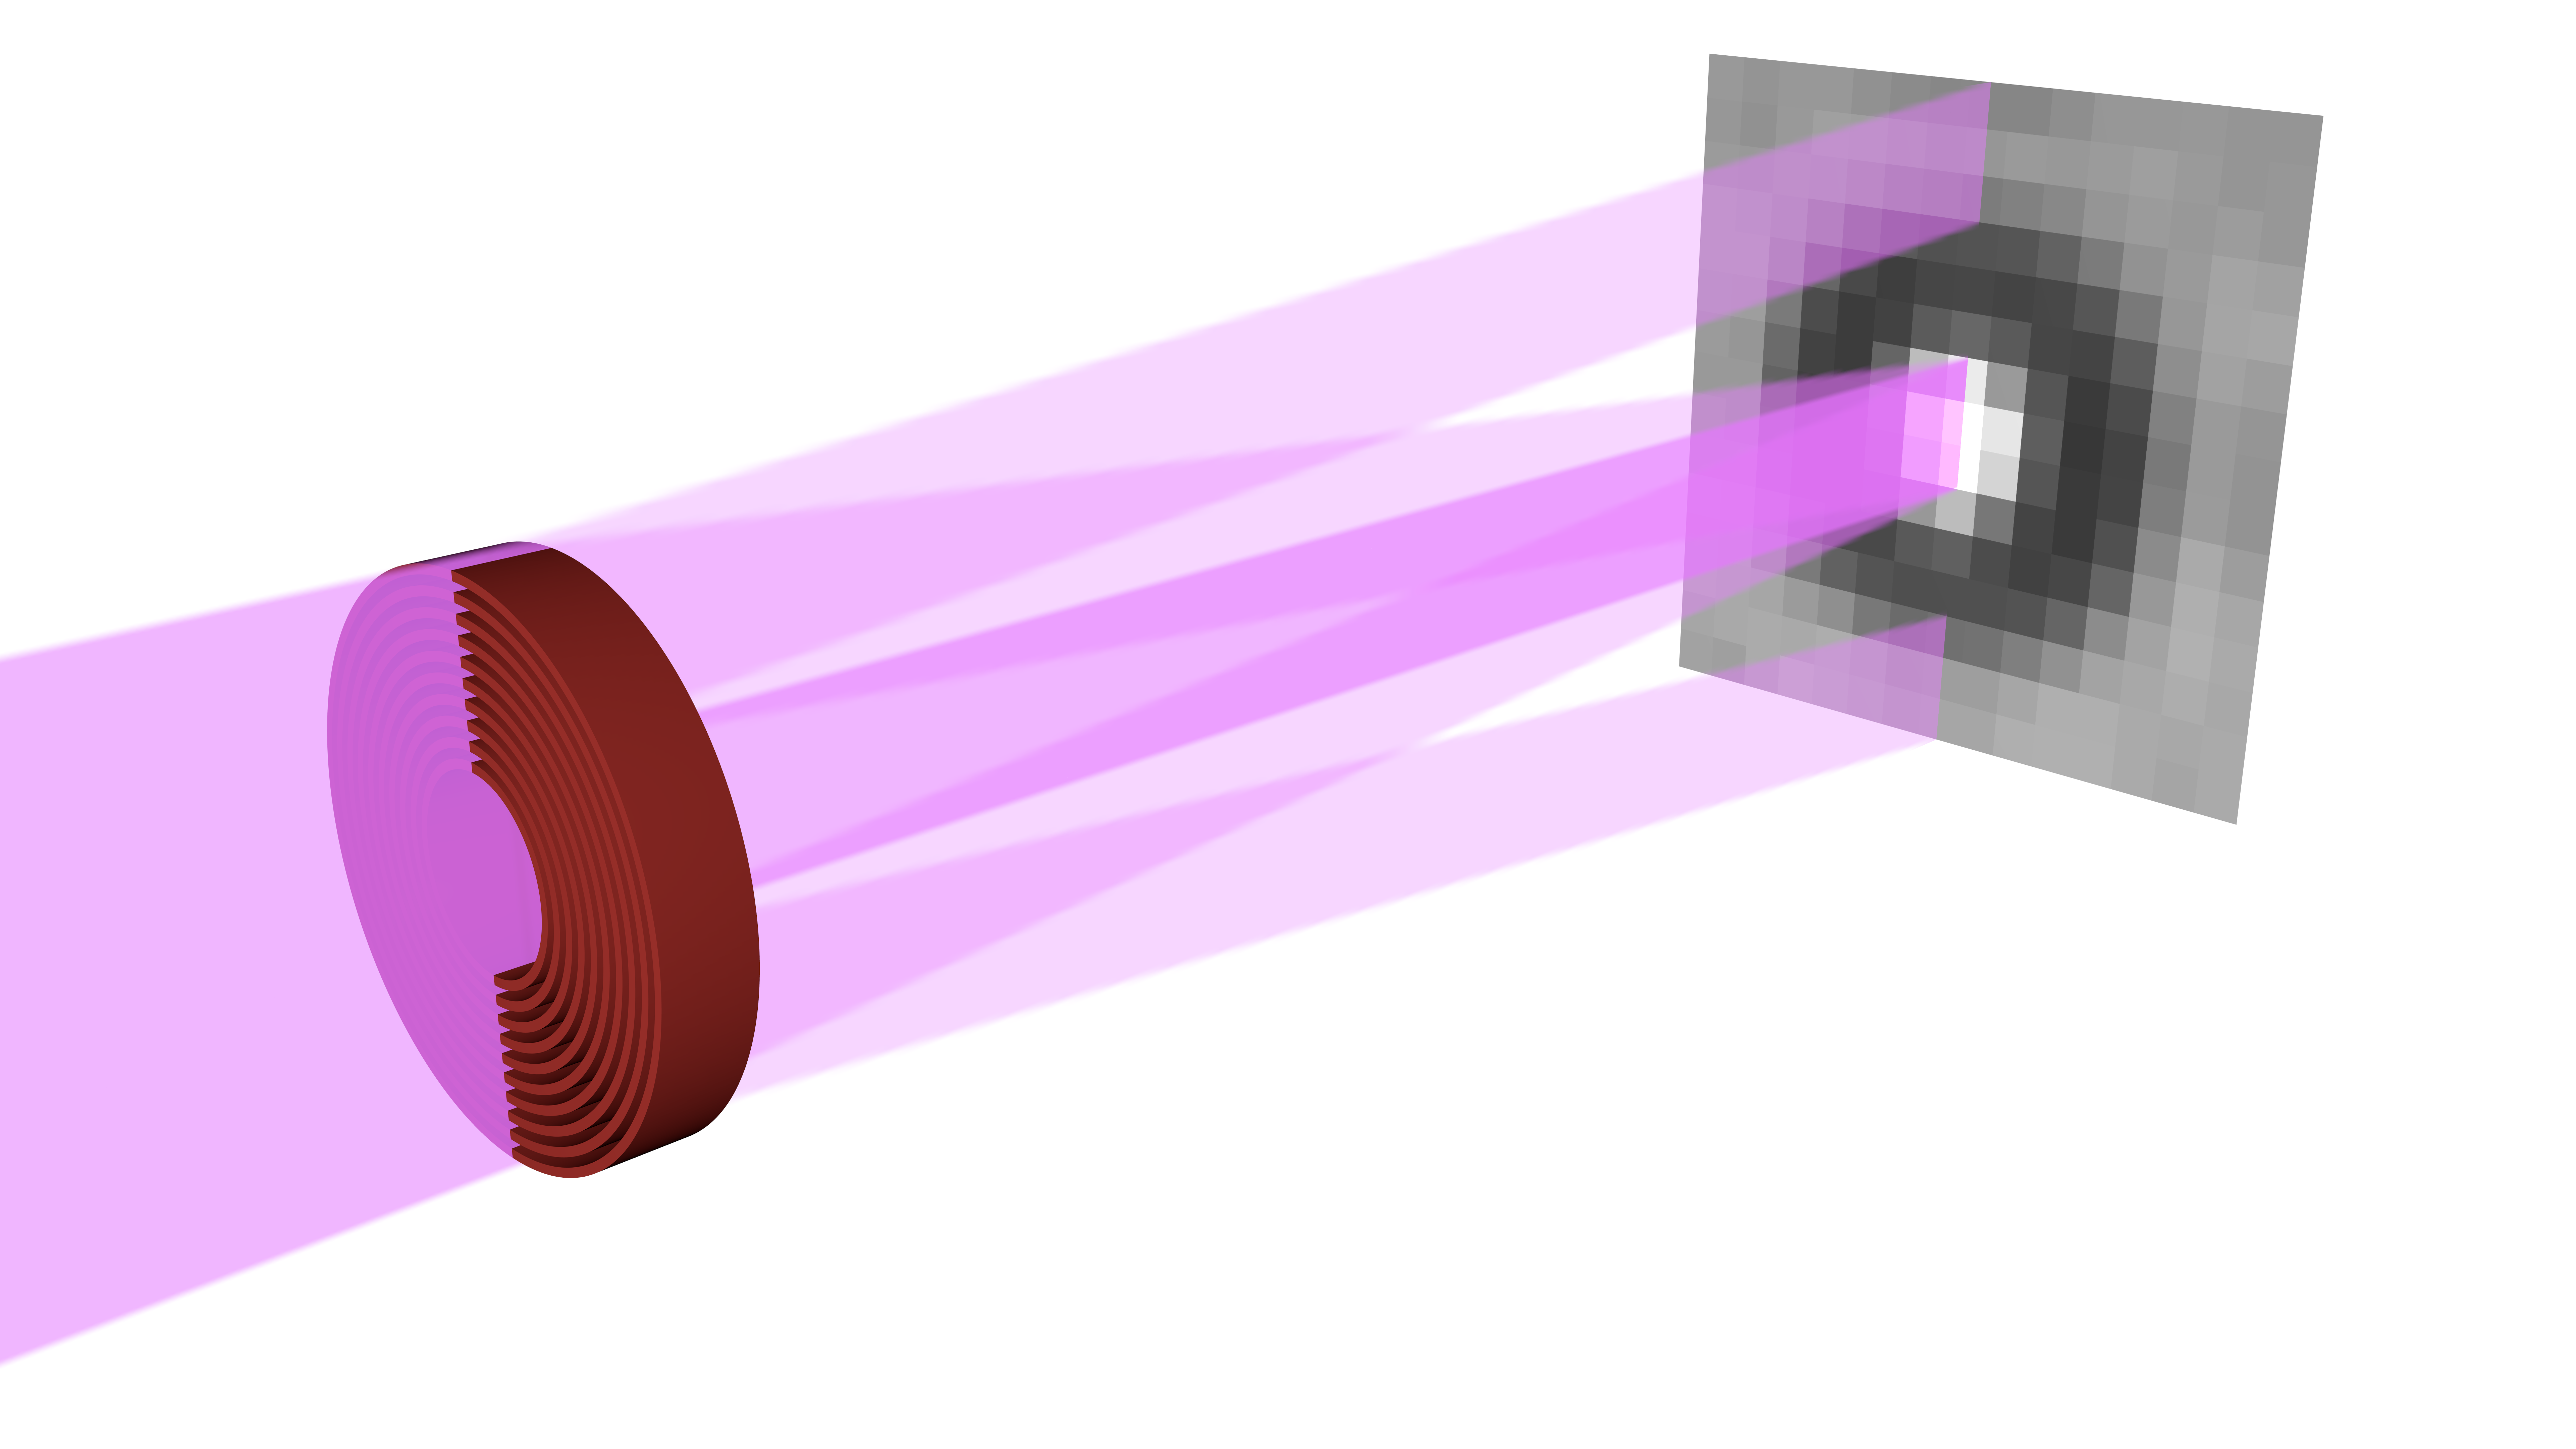
\includegraphics[width=\textwidth]{gfx/omnidirectional/unit_cell.png}
    \caption[Beam splitter grating for the omnidirectional
    interferometer.]{Beam splitter grating for a low coherence
        omnidirectional interferometer. An intensity profile consisting of a
        central maximum
surrounded by a minimum and then a secondary maximum is produced. Designed
by Dr. Kagias~\parencite{kagias2018omnidir}.}
    \label{fig:beam-splitter}
\end{figure}

In order to form this Talbot self-image the coherence requirements of
section~\ref{sec:coherence} have to be satisfied. With reference to
figure~\ref{fig:omnidirectional-lab}, the source size has to be
smaller than
\begin{equation}
    s < \frac{p_2L}{2D}.
    \label{eq:source.size.omnidirectional}
\end{equation}

\begin{figure}[htb]
    \centering
    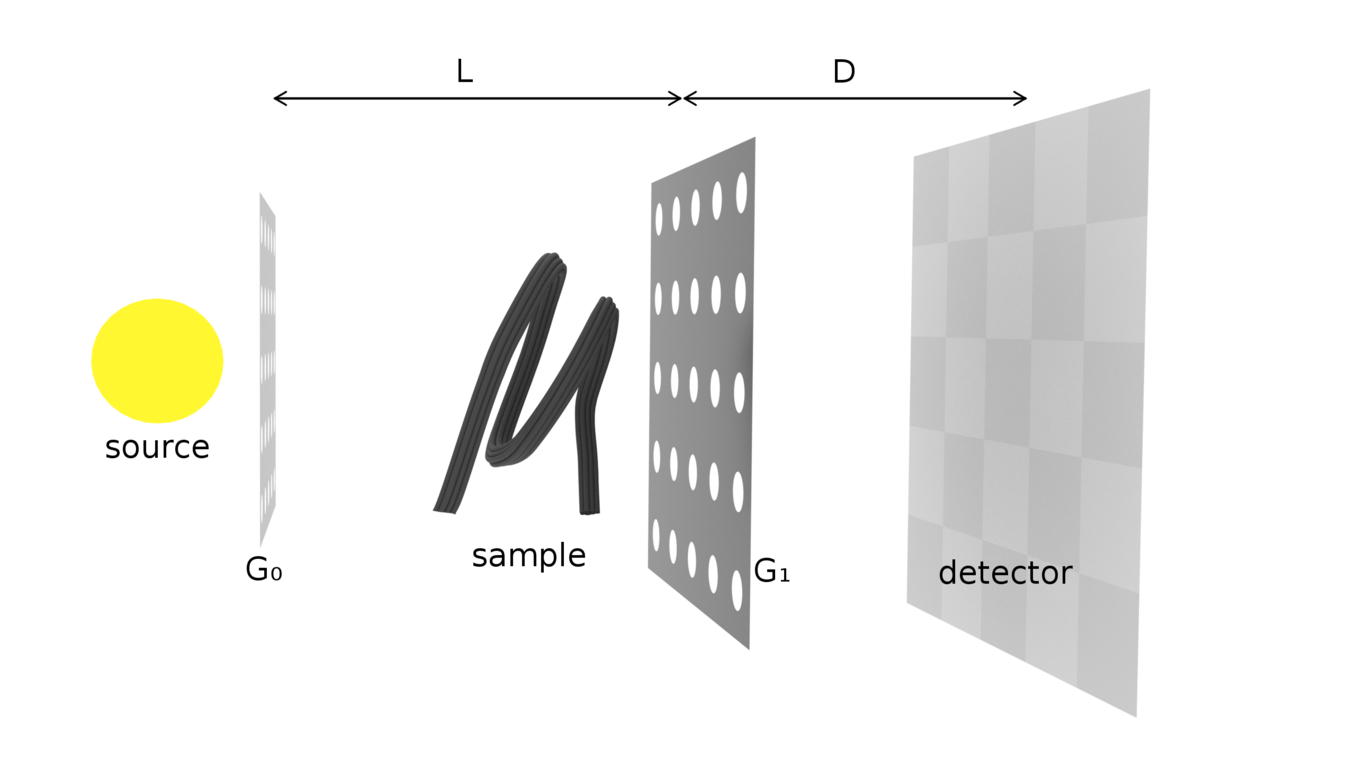
\includegraphics[width=\textwidth]{gfx/omnidirectional/schematic-with-arrows.png}
    \caption[Experimental setup for omnidirectional interferometry on a
    laboratory source.]{Experimental setup for omnidirectional dark-field imaging on a
    laboratory source. The incoherent source is masked by an absorption
grating \G0, similar to Talbot-Lau interferometry, which produces an array
of individually coherent but mutually incoherent
sources~\parencite{kagias2018omnidir}.}
    \label{fig:omnidirectional-lab}
\end{figure}

As in the case of the Talbot interferometer, while this can be achieved in
normal operating conditions for synchrotron experiments, the required
coherence is enforced on the laboratory source with a focal spot size of
\SI{1}{\milli\meter} by introducing an absorption grating \G0. In this case
a two-dimensional array of pinholes with period $p_0 =
\SI{455}{\micro\meter}$ and diameter between $s = \SI{50}{\micro\meter}$ and
$ s = \SI{100}{\micro\meter}$, with a variance given by the penetration of
the laser through the \SI{100}{\micro\meter} thick tungsten
plate. This achieves the required coherence according to
equation~\eqref{eq:source.size.omnidirectional}, while the interference
patterns from different pinhole sources superimpose constructively if
condition~\eqref{eq:p0} is met
\begin{equation}
    p_0 = p_2 \frac{L}{D}\label{eq:p0.omnidirectional},
\end{equation}
where $p_2$ is the magnified period $P$ at the detector plane.

\section{Results}
For our experiment, the beam splitter grating is a silicon grating with
period of \SI{2}{\micro\meter} and a thickness of \SI{37}{\micro\meter},
resulting in a phase shift of $\pi$ at the energy of \SI{30}{\kilo\eV}. The
unit cell size is $P = \SI{300}{\micro\meter}$. The
source is the same as in chapter~\ref{ch:lung-dark-field}, an MXR-225/26
X-ray tube operated at \SI{60}{\kilo\voltpeak} and \SI{10}{\milli\ampere}.
The geometry satisfies
\begin{align*}
    L &= \SI{57}{\centi\meter}\\
    D &= \SI{110}{\centi\meter}.
\end{align*}

The sample is a knot made of carbon fibers, exhibiting a strong
directional scattering signal related to the direction of the fibers. The exposure
time was chosen to be \SI{100}{\second}.
Results are shown in figure~\ref{fig:knot-reconstruction}.

\begin{figure}[htb]
    \centering
    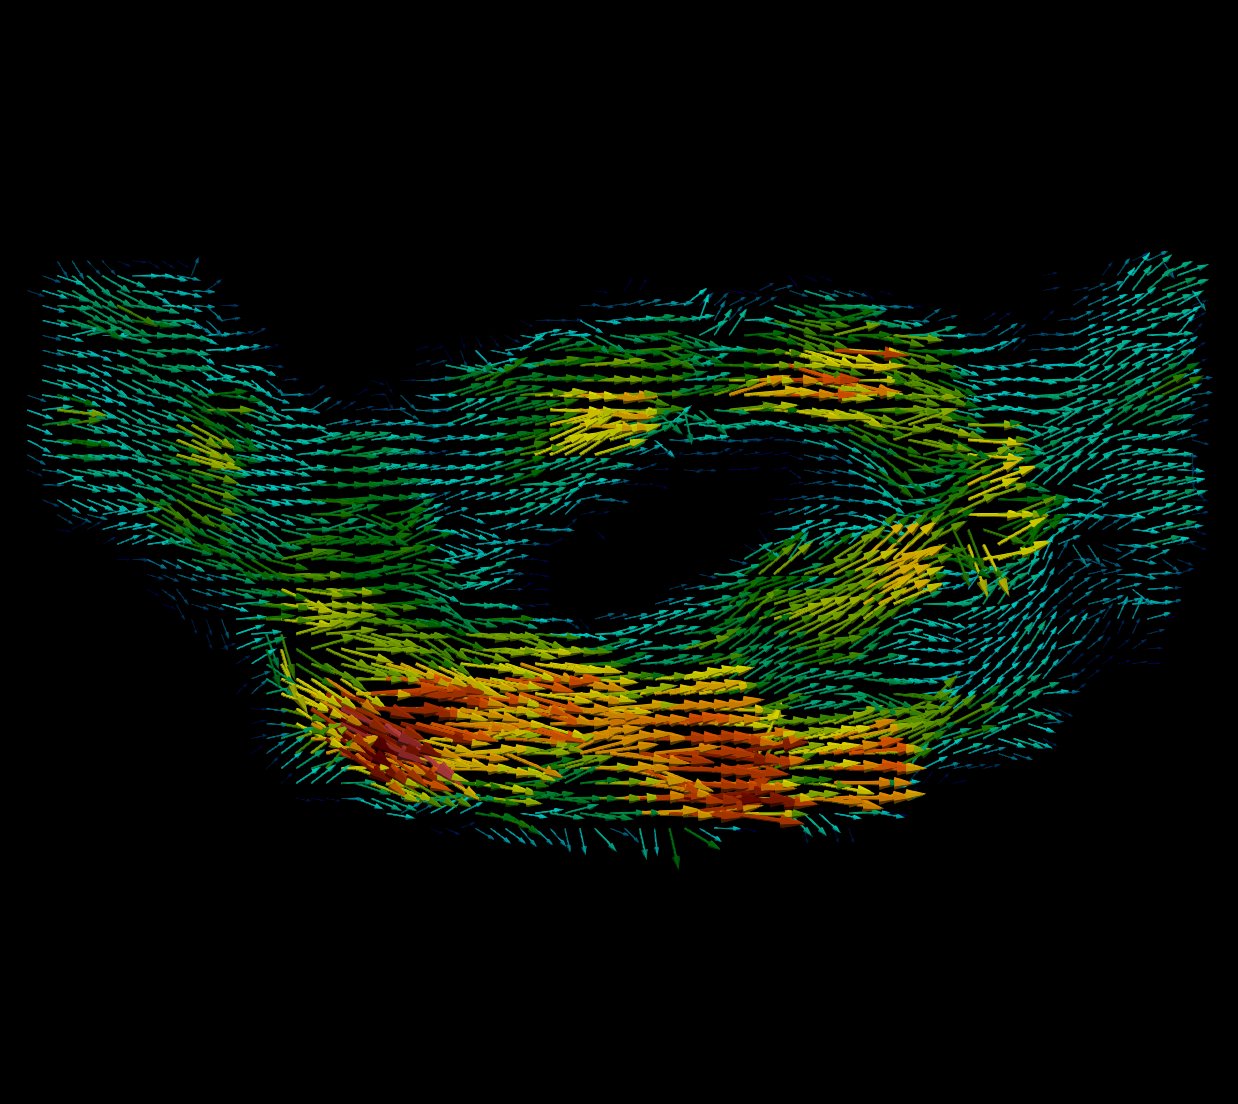
\includegraphics[width=\textwidth]{gfx/omnidirectional/filtered.png}
    \caption[Reconstruction of a carbon fiber knot with omnidirectional
    grating interferometry.]{Knot made of carbon fibers reconstructed with
        equation~\eqref{eq:dark-field-omnidirectional}. The arrow points to
    the spatial direction perpendicular to the largest measured scattering
intensity, its size and colors measure the scattering
strength~\parencite{kagias2018omnidir}.}
    \label{fig:knot-reconstruction}
\end{figure}

It was possible to follow the direction of the alignment of the
carbon fibers around the loop from a single-shot radiography recorded on a
laboratory source.

The performance of this first realization of the interferometer is on par
with the other experiments, with a visibility of the flat image ranging
between \SI{5}{\percent} and \SI{10}{\percent}. The flat image showing the
self image of the unit cells recorded by the detector is shown in
figure~\ref{fig:cells}.

\begin{figure}[htb]
    \centering
    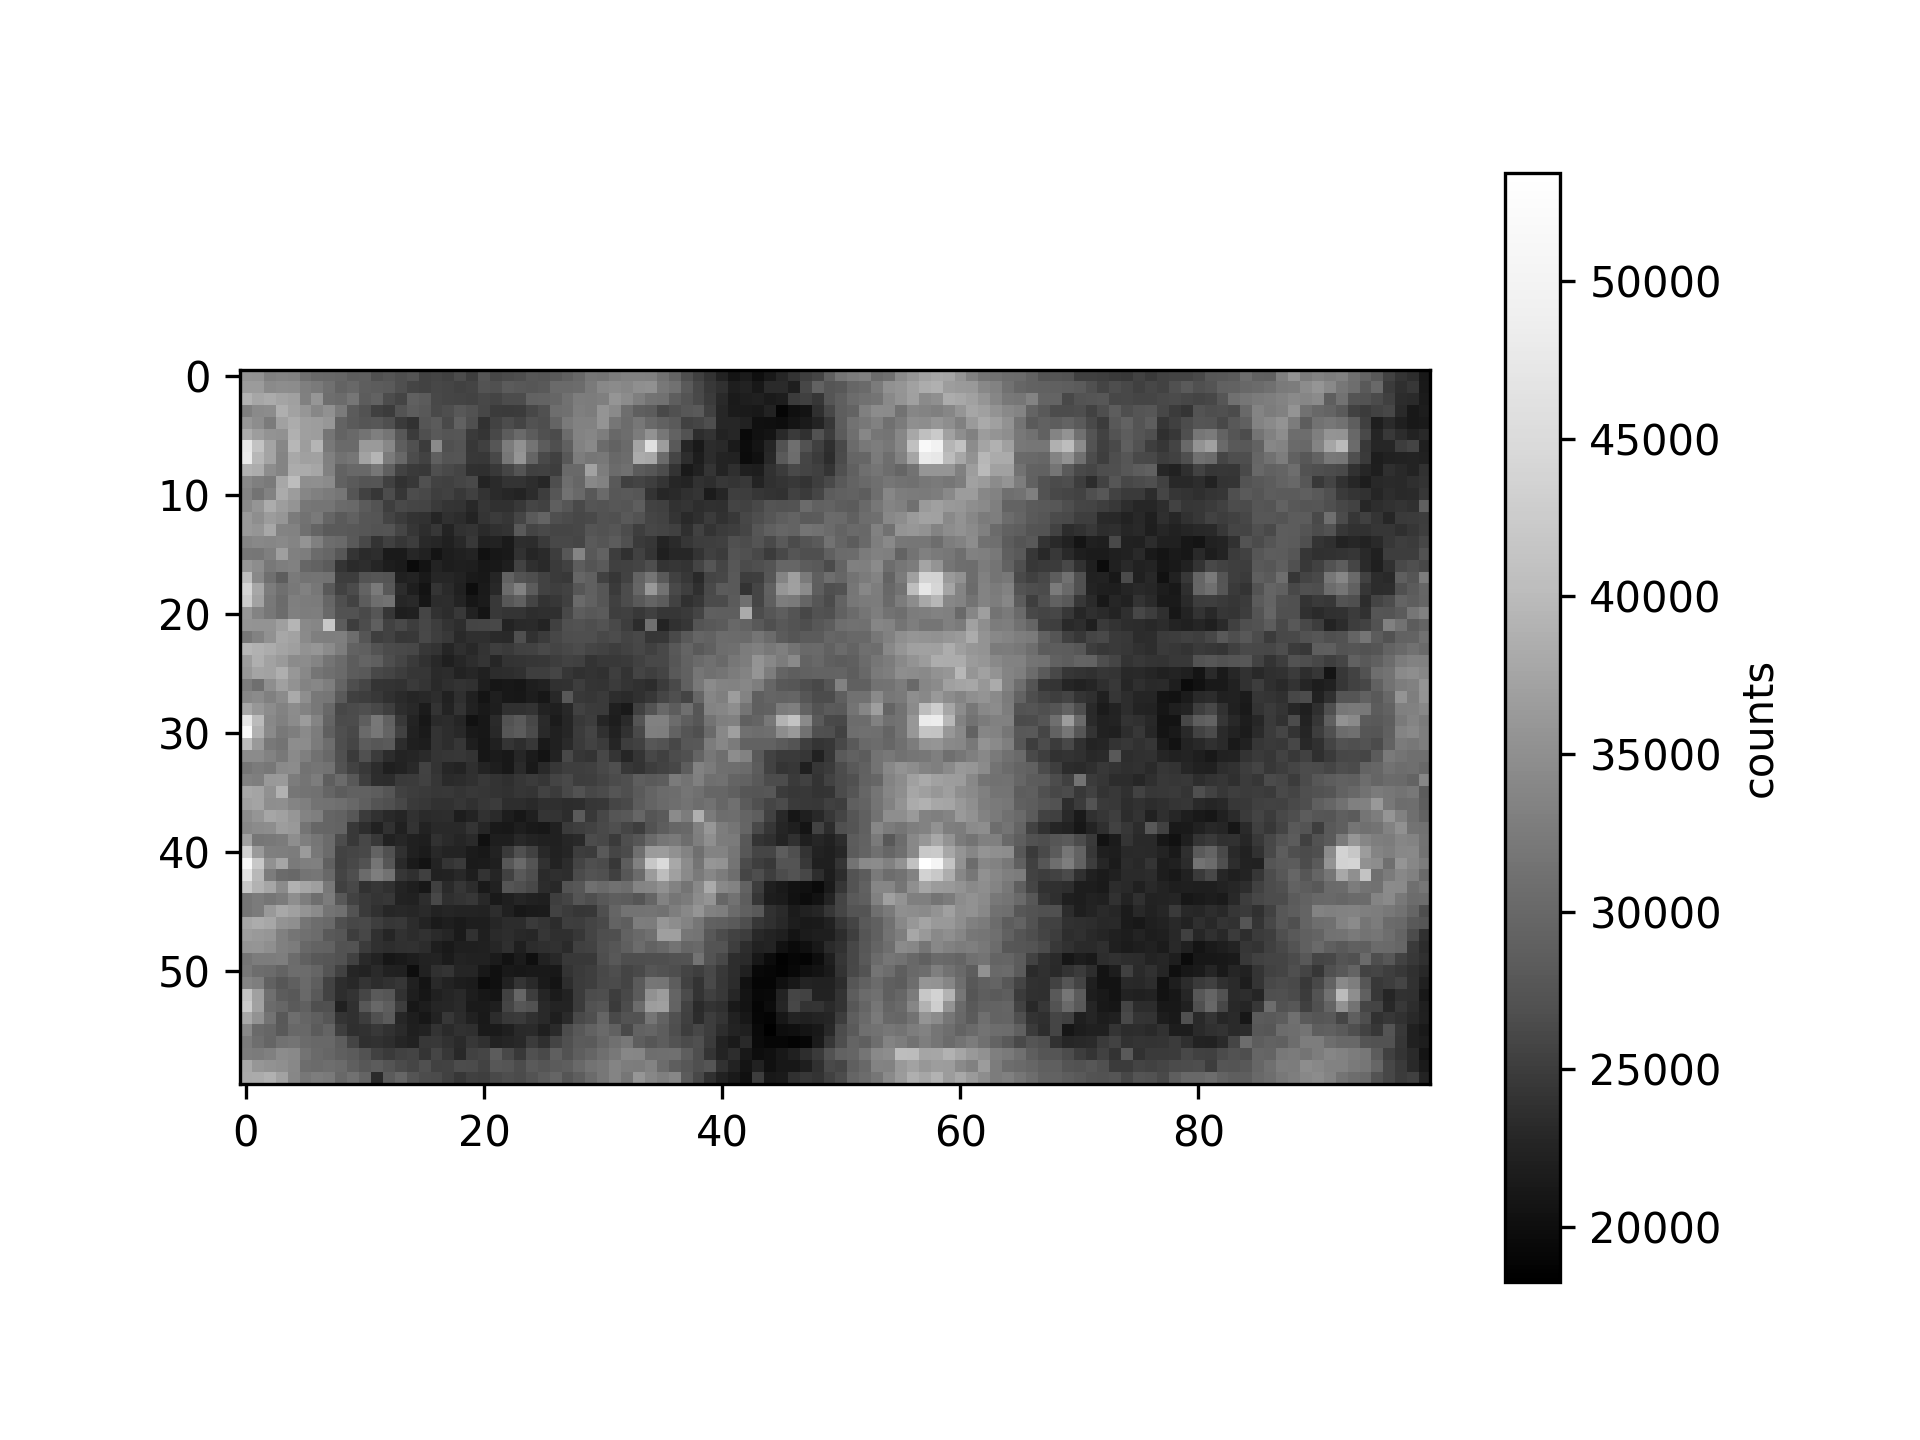
\includegraphics[width=\textwidth]{gfx/omnidirectional/visibility-omnidirectional.png}
    \caption[Self-image of the omnidirectional interference pattern.]{Self-image of the unit cell pattern recorded in the flat image
        for the exposure of~\ref{fig:omnidirectional-lab}. The intensity
        pattern of figure~\ref{fig:beam-splitter} can be recognized.
        Exposure time of~\SI{100}{\second}, the recorded number of counts in
    each pixel is shown.}
    \label{fig:cells}
\end{figure}

\section{Conclusion}
In conclusion, this was the first extension to a laboratory source of
omnidirectional grating interferometry. This technique was developed for
synchrotron experiments by~\cite{PhysRevLett.116.093902}, and could be
applied to a low coherence source with the same principle of Talbot-Lau
interferometry. A pinhole array creates individually coherent sources that
are capable of generating an interference pattern (figure~\ref{fig:cells})
that is large enough to be directly resolved by the detector. The
interference pattern from adjacent pinholes superimpose incoherently but
constructively reinforcing each other if the geometrical
constraint~\eqref{eq:p0} is taken into account. As a result, the strength of
the scattering signal along different directions can be retrieved, with
figure~\ref{fig:knot-reconstruction} showing the dominant direction of the
fibers as they appear to be following the tied cable.
